
\section{解空间}
\label{sec:space-of-solutions}

在这一节中，我们来研究\trFloerEquation{}的解空间
\[
\frac{\partial u}{\partial s}+J(u)\frac{\partial u}{\partial t}+\operatorname{grad}H_t(u)=0\text{，}
\]
我们将采用\cref{fig:w-and-lw-solutions}所表示的两种观点：$W$ 上的方程的解，也就是 $\scr{L}W$ 上的\trVectorField{} $-\operatorname{grad}\scr{A}_H$ 的诸\trTrajectory。

\setcounter{figure}{4}%
\begin{figure}[htbp]
\centering
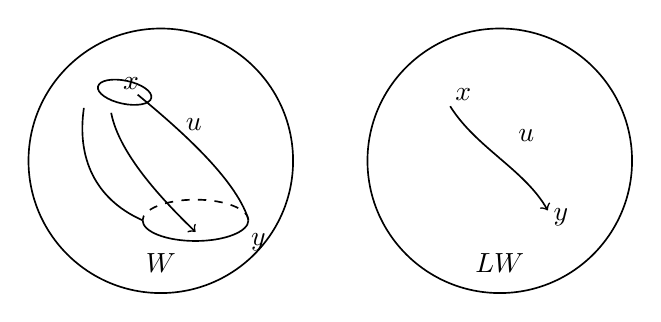
\begin{tikzpicture}[line width=0.6pt,scale=1.05]
  \draw (0,0) circle (1.6);
  \node at (0,-1.24) {$W$};
  \draw[rotate=-12] (-0.6,0.72) ellipse (0.33 and 0.14);
  \draw[dashed] (1.06,-0.72) arc (0:180:0.64 and 0.25);
  \draw (-0.22,-0.72) arc (180:360:0.64 and 0.25);
  \draw (-0.93,0.64) .. controls (-1.03,-0.05) and (-0.72,-0.5) .. (-0.22,-0.72);
  \draw (-0.28,0.80) .. controls (0.18,0.42) and (0.9,-0.2) .. (1.06,-0.71);
  \draw (-0.6,0.58) .. controls (-0.55,0.315) and (-0.375,0.0325) .. (-0.1725,-0.2225);
  \draw[->] (-0.1725,-0.2225) .. controls (0.03,-0.4775) and (0.26,-0.705) .. (0.42,-0.86);
  \node at (-0.36,0.94) {$x$};
  \node at (0.4,0.44) {$u$};
  \node at (1.18,-0.98) {$y$};
  \draw (4.1,0) circle (1.6);
  \node at (4.1,-1.24) {$\scr{L}W$};
  \draw (3.5,0.66) .. controls (3.66,0.405) and (3.885,0.215) .. (4.105,0.026);
  \draw[->] (4.105,0.026) .. controls (4.325,-0.1625) and (4.54,-0.35) .. (4.68,-0.6);
  \node at (3.66,0.8) {$x$};
  \node at (4.42,0.3) {$u$};
  \node at (4.84,-0.68) {$y$};
\end{tikzpicture}
\caption{}
\label{fig:w-and-lw-solutions}
\end{figure}

\subsection{\trEnergy{}的定义}
\label{subsec:definition-energy}

对于无边\trCompact\trManifold{}上的一个函数与一个\trAdapted{}的\trPseudogradient{}场而言，该\trVectorField{}的一切\trTrajectory{}都连接两个\trCriticalPoint。

在我们如今所处的情形里，事情就不再自动如此了。这里有一个类比，用以说明我们可能遭遇到的问题。如果 $V$ 是一个带边\trManifold，那么就可能存在\trPseudogradient{}场的这样一些\trTrajectory：它们到达一个\trCriticalPoint，却并非来自某个\trCriticalPoint（反之亦然），因为它们来自边界。而远离边界的那些\trTrajectory{}确实连接两个\trCriticalPoint。

请注意，在\trCompact\trManifold--\trMorse{}的情形下\footnote{另见第 14 章的练习~27。}，如果 $u\colon\RR\to V$ 是\trDifferential{}方程
\[
\frac{du}{ds}-X(u)=0
\]
的一个解，也就是说，是\trPseudogradient{}场 $X$ 的一条\trTrajectory\footnote{译注：原书方程印作 $\frac{du}{ds}+X(u)=0$，却又随即称 $u$ 是\trPseudogradient{}场 $X$ 的一条\trTrajectory；但按本书的约定（第 2 章），\trAdapted{}于 $f$ 的\trPseudogradient{}满足 $df(X)\le 0$（等号仅在\trCriticalPoint{}处成立），方程 $\frac{du}{ds}+X(u)=0$ 的解实为 $-X$ 的\trTrajectory，沿之 $f$ 自 $a$ 升至 $b$，于是 $E(u)=f(a)-f(b)\le 0$，与下句“定义中的那个负号保证\trEnergy{}是正的、$a$ 位于 $b$ 之上”直接矛盾。方程疑应作 $\frac{du}{ds}-X(u)=0$：此时 $u$ 才是 $X$ 的\trTrajectory，$f$ 沿之递减，$E(u)=f(a)-f(b)>0$，全段自洽；此处径改。——译者注}，那么我们就可以定义它的\trEnergy
\[
E(u)=-\int_{-\infty}^{+\infty}u^\star df\text{。}
\]
如果 $u$ 连接两个\trCriticalPoint{} $a$ 与 $b$，即 $\lim_{s\to-\infty}u(s)=a$ 而 $\lim_{s\to+\infty}u(s)=b$，那么这个\trEnergy{}就简单地是
\[
E(u)=f(a)-f(b)
\]
（定义中的那个负号保证了\trEnergy{}是正的，因为对函数 $f$ 而言，点 $a$ 位于点 $b$ 之上）。

\begin{remark}[闭形式]\label{thm:closed-forms-remark}
在这个定义中，可以把\trExact{}形式 $df$ 换成一个\trClosed{} $1$-形式 $\alpha$。我们将在 §6.7 中看到，此时仍然可以构造出一个\trAdapted{}的\trPseudogradient{}场，但显而易见，并非这样一个\trVectorField{}的一切\trTrajectory{}都连接这个形式的零点。在这种情形下，有限\trEnergy{}的那些\trTrajectory{}恰恰就是连接这个形式两个零点的\trTrajectory。这也正是\trActionFunctional{}的情形。
\end{remark}

对于我们这里感兴趣的\trActionFunctional{}的情形，我们以类似的方式来定义一个解的\trEnergy。这归结为沿一个解积分其\trGradient{}范数的平方（“\trEnergy”之名即由此而来）：
\[
\begin{aligned}
E(u)&=-\int_{-\infty}^{+\infty}\frac{d}{ds}\scr{A}_H(u(s))\,ds\\
&=-\int_{-\infty}^{+\infty}-\|\operatorname{grad}\scr{A}_H\|^2\,ds\\
&=\int_{-\infty}^{+\infty}\Bigl(\int_{S^1}\Bigl|\frac{\partial u}{\partial s}\Bigr|^2\,dt\Bigr)ds\\
&=\frac{1}{2}\int_{-\infty}^{+\infty}\Bigl(\int_{S^1}\Bigl(\Bigl|\frac{\partial u}{\partial s}\Bigr|^2+\Bigl|\frac{\partial u}{\partial t}-X_t(u)\Bigr|^2\Bigr)dt\Bigr)ds\text{。}
\end{aligned}
\]
请注意，由于 $u$ 是一个解，积分中的两项相等，于是
\[
E(u)=\int_{\RR\times S^1}\Bigl|\frac{\partial u}{\partial s}\Bigr|^2\,ds\,dt\text{。}
\]

\begin{remark}\label{thm:energy-solution-remarks}
\begin{enumerate}[label=(\arabic*)]
\item \trEnergy{}是正的。
\item 一个解的\trEnergy{}为零，当且仅当 $\partial u/\partial s$ 为零，也就是说 $u$ 不依赖于 $s$……并且 $u$ 是\trFloerEquation{}的一个解，也就是说，当且仅当 $u$ 是\trActionFunctional{} $\scr{A}_H$ 的一个\trCriticalPoint。
\item 如果所论的解 $u$ 连接两个\trCriticalPoint，也就是说，如果存在 $\scr{A}_H$ 的\trCriticalPoint{} $x$ 与 $y$，使得
\[
\lim_{s\to-\infty}u_s(t)=x\text{，}\qquad \lim_{s\to+\infty}u_s(t)=y\text{，}
\]
那么
\[
E(u)=\scr{A}_H(x)-\scr{A}_H(y)<+\infty\text{。}
\]
连接两个\trCriticalPoint{}的那些解都具有有限的\trEnergy。
\end{enumerate}
\end{remark}

因此，让我们来考虑由
\[
\scr{M}=\Bigl\{u\colon\RR\times S^1\to W \ \Bigm|\ u\ \text{是一个有限\trEnergy{}的\trContractible{} $\cC^\infty$ 解}\Bigr\}
\]
所定义的空间 $\scr{M}$。

为了免于此空间上\trTopology{}定义的种种麻烦，我们将总是把\trCompact\trSymplectic\trManifold{} $W$ 看成\trEmbedding{}于一个\trEuclidean{}空间 $\RR^m$ 之中（$m$ 充分大）。对于从 $S^1$ 到 $\RR^m$ 的映射，我们将使用 $\cC^\infty$ \trTopology；而对于 $\RR\times S^1$ 的\trCompact{}子集，则使用 $\cC^\infty$ \trUniformConvergence{}\trTopology，并采用如下记号：$\cC^\infty(S^1;W)$，$\cC^\infty(S^1;\RR^m)$，$\cC^\infty_{\mathrm{loc}}(\RR\times S^1;W)$，$\cC^\infty_{\mathrm{loc}}(\RR\times S^1;\RR^m)$。

一个强有力的\trEllipticRegularity{}结果使我们得以证明下述命题所包含的那个本质性质。

\begin{proposition}\label{thm:solution-smoothness-regularity}
\trFloerEquation{}的每一个 $\cC^1$ 类的解都是 $\cC^\infty$ 类的。此外，在 $\scr{M}$ 上，诸\trTopology{} $\cC^0_{\mathrm{loc}}$、$\cC^1_{\mathrm{loc}}$ 与 $\cC^\infty_{\mathrm{loc}}$ 相重合。
\end{proposition}

\begin{proof}
这个证明是\trEllipticRegularity{}引理（引理~12.1.1）与命题~6.6.2 的一个直接推论。
\end{proof}

这个空间 $\scr{M}$ 的一个重要性质是它的\trCompact{}性。这是一个本质性的性质，我们将在后面（在 §6.6 中）证明它，现在先把它陈述出来。

\begin{theorem}[\trGromov{}\trCompact{}性]\label{thm:gromov-compactness-theorem}
设\trCompact\trSymplectic\trManifold{} $(W,\omega)$ 满足\cref{thm:symplectic-asphericity}，即
\[
\forall f\colon S^2\longrightarrow W,\qquad \int_{S^2}f^\star\omega=0\text{。}
\]
那么 $\scr{M}$ 在 $\cC^\infty_{\mathrm{loc}}(\RR\times S^1,W)$ 中是\trCompact{}的。
\end{theorem}

\begin{remark}\label{thm:work-in-moduli-remark}
在这整整一节中，我们都将在 $\scr{M}$ 中工作。我们尚未证明\trFloerEquation{}有任何解（当心，这并不是一个\trCauchy{}问题）。
\end{remark}

\subsection{有限\trEnergy{}的解趋于\trCriticalPoint}
\label{subsec:finite-energy-tends-critical}

我们将证明\cref{thm:energy-solution-remarks}最后一条的一个逆命题，也就是下述定理。

\begin{theorem}\label{thm:trajectories-tend-critical-points}
设 $X_t$ 的一切\trPeriodic\trTrajectory{}都是\trNondegenerate{}的；那么对每个 $u\in\scr{M}$，都存在 $\scr{A}_H$ 的两个\trCriticalPoint{} $x$ 与 $y$，使得
\[
\lim_{s\to-\infty}u(s,\cdot)=x\text{，}\qquad \lim_{s\to+\infty}u(s,\cdot)=y
\]
在 $\cC^\infty(S^1;W)$ 中成立。此外，
\[
\lim_{s\to\pm\infty}\frac{\partial u}{\partial s}(s,t)=0
\]
关于 $t$ 一致。
\end{theorem}

\textbf{沿一条\trTrajectory，函数趋于一个\trCriticalValue。\trEnergy{}的\trUniform{}界}

让我们先来证明一个较弱的结果。

\begin{proposition}\label{thm:action-tends-critical-values}
设 $u\in\scr{M}$。那么存在 $\scr{A}_H$ 的两个\trCriticalPoint{} $x$ 与 $y$，使得
\[
\lim_{s\to-\infty}\scr{A}_H(u_s)=\scr{A}_H(x)\text{，}\qquad \lim_{s\to+\infty}\scr{A}_H(u_s)=\scr{A}_H(y)\text{。}
\]
\end{proposition}

\begin{remark}\label{thm:critical-points-nonempty-remark}
这条命题的一个显而易见的推论就是：如果 $\scr{M}$ 非空，那么 $\scr{A}_H$ 有\trCriticalPoint。
\end{remark}

\begin{corollary}\label{thm:uniform-energy-bound}
存在一个实数 $C>0$，使得对每个 $u\in\scr{M}$，都有
\[
-C\le\scr{A}_H(u)\le C\quad\text{并且}\quad 0\le E(u)\le C\text{。}
\]
\end{corollary}

\begin{proof}
$\scr{A}_H$ 的\trCriticalPoint{}所成之集是有限的（并且非空），故 $\scr{A}_H$ 在这个集合上\trBounded\footnote{另见第 14 章的练习~30，那里去掉了\trNondegenerate{}性假设。}。为得出结论，我们还需用到：
\begin{itemize}
\item $s\mapsto\scr{A}_H(u_s)$ 是递减的；
\item 并且，对 $\scr{M}$ 中的 $u$ 与\cref{thm:action-tends-critical-values}陈述中那样的\trCriticalPoint{} $x$、$y$（也就是说，使得 $\scr{A}_H(u_s)$ 从 $\scr{A}_H(x)$ 走到 $\scr{A}_H(y)$ 的那些），我们有
\[
E(u)=\scr{A}_H(x)-\scr{A}_H(y)\text{。}\qedhere
\]
\end{itemize}
\end{proof}

\begin{proof}[\cref{thm:action-tends-critical-values}的证明]
我们将把自己限制在 $s\to+\infty$ 的情形，因为另一种情形是类似的。（一个实变量的那个实）函数 $s\mapsto\scr{A}_H(u_s)$ 是递减的（它的导数是\trGradient{}范数的负值，因而是负的）。因此，只需证明：存在 $\scr{A}_H$ 的一个\trCriticalPoint{} $y$ 与一列趋于无穷的实数 $s_k$，使得
\[
\lim_{k\to+\infty}\scr{A}_H(u_{s_k})=\scr{A}_H(y)\text{。}
\]
我们将分三步来证明这一点：
\begin{enumerate}[label=(\arabic*)]
\item 存在序列 $s_k$，使得 $u_{s_k}$ 对于 $\cC^0(S^1;W)$ \trTopology{}\trConvergence{}到一个极限 $y$。
\item 这个极限 $y$ 是 $\cC^\infty$ 的，并且是 $\scr{A}_H$ 的一个\trCriticalPoint。
\item $\scr{A}_H(u_{s_k})$ 的确趋于 $\scr{A}_H(y)$。
\end{enumerate}

\textbf{第一步。}

设 $u\in\scr{M}$。由于
\[
\int_{-\infty}^{+\infty}\Bigl(\int_{S^1}\Bigl|\frac{\partial u}{\partial t}-X_t(u)\Bigr|^2\,dt\Bigr)ds<+\infty\text{，}
\]
$\partial u/\partial t-X_t(u)$ 的 $L^2$ 范数的积分是有限的。于是存在序列 $(s_k)$，满足 $\lim_{k\to\infty}s_k=+\infty$（相应地 $-\infty$），使得
\[
\lim_{k\to\infty}\Bigl\|\frac{\partial u}{\partial t}(s_k,t)-X_t(u(s_k,t))\Bigr\|_{L^2}=0\text{。}
\]
为简化记号，令 $u_{s_k}=u_k$。而为了帮助我们理解这一点，请注意，我们刚才写下的那些积分中的范数，原则上是由 $J$ 定义的范数……但是\trManifold{} $W$ 是\trCompact{}的且\trEmbedding{}于 $\RR^m$ 中，于是这个\trEmbedding{}的\trTangentMap{}的算子范数在源头处被由 $J$ 定义的范数所控制、在靶处被\trEuclidean{}范数所控制，这就蕴含着我们可以用\trEuclidean{}范数来工作。

于是我们有
\[
\lim_{k\to+\infty}\int_0^1\|\dot{u}_k-X_t(u_k)\|^2\,dt=0\text{，}
\]
也就是说，
\[
\lim_{k\to+\infty}\|\dot{u}_k-X_t(u_k)\|_{L^2(S^1;\RR^m)}=0\text{。}
\]
由于\trManifold{} $W$ 是\trCompact{}的，$X_t(u(s_k,t))$ 是\trBounded{}的，于是存在 $B>0$ 使得
\[
\|\dot{u}_k\|_{L^2}\le B\text{。}
\]
诸 $u_k$ 所成之族因而是\textbf{\trEquicontinuity}（equicontinuity）的：
\[
\begin{aligned}
\|u_k(t_1)-u_k(t_0)\|&=\Bigl\|\int_{t_0}^{t_1}\dot{u}_k(t)\,dt\Bigr\|\\
&\le\int_{S^1}\mathbf{1}_{[t_0,t_1]}\|\dot{u}_k\|\\
&\le\sqrt{t_1-t_0}\,\|\dot{u}_k\|_{L^2}\quad\text{（由\trCauchy--\trSchwarz{}不等式）}\\
&\le B\sqrt{t_1-t_0}\text{。}
\end{aligned}
\]
$u_k$ 的像含于\trCompact{}的 $W$ 之中。于是序列 $u_k$ 是\textbf{\trArzelaAscoliTheorem}（Arzelà--Ascoli theorem）的一个候选\footnote{参见\cref{sec:appC-arzela-ascoli}。}，并且我们由此得出结论：序列 $u_k$ 在 $\cC^0(S^1;\RR^m)$ \trTopology{}下、也就是说在 $\cC^0(S^1;W)$ \trTopology{}下有一个极限 $y$。至此，这个证明的第一步完成。

\textbf{第二步。}

让我们来证明，极限 $y$ 是 $\cC^\infty$ 的，并且是\trHamiltonian{}系统 $\dot{x}=X_t(x)$ 的一个解。

\begin{lemma}\label{thm:limit-integral-formula}
极限 $y$ 满足
\[
y(t)-y(0)=\int_0^tX_\tau(y(\tau))\,d\tau\text{。}
\]
\end{lemma}

所预期的结果由这条引理而来，因为它蕴含：由于 $y$ 连续，故它是 $\cC^1$ 的，从而是 $\cC^2$ 的……并且它是一个解。因而它是 $\cC^\infty$ 的（这显然是一例“自举”\footnote{“自举”原文作 bootstrapping，本义说的是只靠自己拉住自己的靴带、就能把自己提起来腾空的本事。在本书中，它一般指的则是法国人所谓的“\trEllipticRegularity”：偏\trDifferential{}方程的一个在\trDistribution{}意义下的\textbf{\trWeakSolution}（weak solution）自动地就是一个 $\cC^\infty$ 函数。参见附录 C。}）。这样，我们便在 $\cC^0$ 意义下\trConvergence{}到一个 $\cC^\infty$ 解。

\begin{proof}[\cref{thm:limit-integral-formula}的证明]
让我们来考察这个差
\[
y(t)-y(0)-\int_0^tX_\tau(y(\tau))\,d\tau=\lim_{k\to+\infty}\Bigl(u_k(t)-u_k(0)-\int_0^tX_\tau(y(\tau))\,d\tau\Bigr)
\]
（这就是身处 $\RR^m$ 这个\trVectorSpace{}之中的好处）。它也等于
\[
\begin{aligned}
y(t)-y(0)-\int_0^tX_\tau(y(\tau))\,d\tau
&=\lim_{k\to+\infty}\Bigl(\int_0^t\dot{u}_k(\tau)\,d\tau-\int_0^tX_\tau(y(\tau))\,d\tau\Bigr)\\
&=\lim_{k\to+\infty}\Bigl(\int_0^t\dot{u}_k(\tau)-X_\tau(u_k(\tau))\,d\tau\Bigr)\\
&\qquad+\lim_{k\to+\infty}\Bigl(\int_0^t\left(X_\tau(u_k(\tau))-X_\tau(y(\tau))\right)d\tau\Bigr)\text{。}
\end{aligned}
\]
这两项都趋于 $0$。$u_k$ 在 $\cC^0$ 意义下趋于 $y$ 这一事实蕴含第二项趋于 $0$。对于第一项，我们利用 $\|\dot{u}_k-X_\tau(u_k)\|_{L^2}$ 趋于 $0$ 这一事实以及\trCauchy--\trSchwarz{}不等式，这就给出\footnote{译注：原书此引理的陈述与证明中 $X_t$／$X_\tau$ 混用（积分变量为 $\tau$，被积\trVectorField{}却多印作 $X_t$，仅末行左端作 $X_\tau$），且末行中段积分缺 $d\tau$；按积分变量为 $\tau$ 疑均应作 $X_\tau$；此处径改统一并补齐。——译者注}
\[
\Bigl|\int_0^t(\dot{u}_k(\tau)-X_\tau(u_k))\,d\tau\Bigr|=\Bigl|\int_0^1\mathbf{1}_{[0,t]}(\dot{u}_k-X_\tau(u_k))\,d\tau\Bigr|\le\sqrt{t}\,\|\dot{u}_k-X_\tau(u_k)\|_{L^2}\text{，}
\]
而它的确趋于 $0$。
\end{proof}

$\cC^1$（乃至 $\cC^\infty$）的\trConvergence{}由这些论证得出。

\textbf{第三步。}

让我们来证明 $\scr{A}_H(u_k)$ 趋于 $\scr{A}_H(y)$。\trHamiltonian{}的积分部分显然不带来任何困难，并且
\[
\int_0^1H_t(u_k)\,dt\ \text{趋于}\ \int_0^1H_t(y(t))\,dt
\]
因为 $u_k$ 对于 $\cC^0$ \trTopology{}趋于 $y$。

于是让我们来考察\trActionFunctional{}的另外一部分。为此，我们选取 $u_k$ 与 $y$（各自）到\trDisk{}上的扩张 $\widetilde{u}_k$ 与 $\widetilde{u}_y$。我们必须证明
\[
\lim_{k\to+\infty}\Bigl(\int_{D^2}\widetilde{u}_k^\star\omega-\int_{D^2}\widetilde{u}_y^\star\omega\Bigr)=0\text{。}
\]
如果\trForm{} $\omega$ 是\trExact{}的，$\omega=d\lambda$，那么我们就会有
\[
\begin{aligned}
\int_{D^2}\widetilde{u}_k^\star\omega-\int_{D^2}\widetilde{u}_y^\star\omega
&=\int_{S^1}u_k^\star\lambda-\int_{S^1}y^\star\lambda\\
&=\int_0^1(\lambda(\dot{u}_k)-\lambda(\dot{y}))\,dt\\
&=\int_0^1\lambda(\dot{u}_k-X_t(u_k))\,dt+\int_0^1\lambda(X_t(u_k)-X_t(y))\,dt\text{。}
\end{aligned}
\]
最后一个积分趋于 $0$，因为 $u_k$ 趋于 $y$。对于第一个积分，我们有\footnote{译注：原书此式积分号内印作 $\lambda(\dot{u}_k)-X_t(u_k)$；据右端范数 $\|\dot{u}_k-X_t(u_k)\|_{L^1}$ 与上式，被积函数应为 $\lambda(\dot{u}_k-X_t(u_k))$；此处径改。——译者注}
\[
\Bigl|\int_0^1\lambda(\dot{u}_k-X_t(u_k))\,dt\Bigr|\le\sup\|\lambda\|\,\|\dot{u}_k-X_t(u_k)\|_{L^1}
\]
……对于这个 $L^1$ 范数，由于 $S^1$ 的\trCompact{}性，我们可以把它换成 $L^2$ 范数。所预期的结果随之而来，因为这个 $L^2$ 范数趋于 $0$，正如我们在第一步中所指出的。

只不过，$W$ 是\trCompact{}的，因而 $\omega$ 并非\trExact{}。我们选取 $W$ 中 $y$ 的像的一个邻域 $\scr{U}$，使它收缩到 $y$ 上，从而 $\omega|_{\scr{U}}$ 是\trExact{}的。对充分大的 $k$，$u_k$ 的像含于 $\scr{U}$ 之中。接着，我们通过\trGluing{}造出一个 $S^2$ \trSphere：
\begin{itemize}
\item 一个柱面 $C\to\scr{U}$，它是 $u_k$ 与 $y$ 之间的一个\trHomotopy，并且含于 $\scr{U}$ 之中；
\item 以 $y$ 为边缘的\trDisk{} $\widetilde{u}_y$；
\item 以 $u_k$ 为边缘的\trDisk{} $\widetilde{u}_k$。
\end{itemize}
根据\cref{thm:symplectic-asphericity}——即 $\omega$ 在诸\trSphere{}上的积分为零——显然，
\[
\int_{D^2}\widetilde{u}_k^\star\omega-\int_{D^2}\widetilde{u}_y^\star\omega
\]
这个差就是 $\omega$ 在柱面 $C$ 上的积分，在这个柱面上 $\omega$ 是\trExact{}的，并且前面的计算在此有效。
\end{proof}

\textbf{诸\trTrajectory{}趋于\trCriticalPoint。}

让我们现在来证明诸\trTrajectory{}趋于\trCriticalPoint，也就是说，证明\cref{thm:trajectories-tend-critical-points}。要点在于空间 $\scr{M}$ 是\trCompact{}的这一事实（\cref{thm:gromov-compactness-theorem}，我们将在后面证明它）。

\begin{figure}[htbp]
\centering
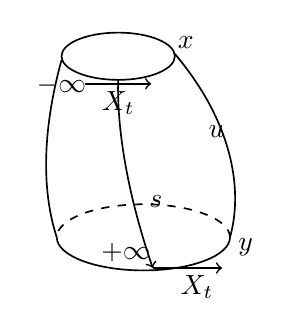
\begin{tikzpicture}[line width=0.6pt,scale=1.0]
  \draw (0.3,1.35) ellipse (0.72 and 0.30);
  \draw[dashed] (1.72,-0.95) arc (0:180:1.1 and 0.42);
  \draw (-0.48,-0.95) arc (180:360:1.1 and 0.42);
  \draw (-0.42,1.30) .. controls (-0.68,0.35) and (-0.66,-0.4) .. (-0.48,-0.95);
  \draw (1.02,1.38) .. controls (1.72,0.55) and (1.9,-0.3) .. (1.72,-0.95);
  \draw (0.3,1.05) .. controls (0.29,0.7) and (0.3275,0.3125) .. (0.404,-0.0925);
  \draw[->] (0.404,-0.0925) .. controls (0.48,-0.4975) and (0.595,-0.92) .. (0.74,-1.34);
  \draw[->] (-0.12,1.0) -- (0.72,1.0);
  \draw[->] (0.74,-1.34) -- (1.62,-1.34);
  \node at (1.16,1.52) {$x$};
  \node at (1.92,-1.08) {$y$};
  \node at (1.55,0.4) {$u$};
  \node at (-0.42,0.98) {$-\infty$};
  \node at (0.3,0.76) {$X_t$};
  \node at (0.4,-1.14) {$+\infty$};
  \node at (1.3,-1.58) {$X_t$};
  \node at (0.78,-0.5) {$s$};
\end{tikzpicture}
\caption{}
\label{fig:cylinder-trajectory-schematic}
\end{figure}

于是让我们假定 $X_t$ 的一切\trPeriodic\trTrajectory{}都是\trNondegenerate{}的。

\begin{lemma}\label{thm:finitely-many-critical-points}
在\trNondegenerate{}性假设之下，$\scr{A}_H$ 的\trCriticalPoint——或者说 $X_t$ 的\trPeriodic\trTrajectory——只有有限多个。
\end{lemma}

\begin{proof}
这些\trCriticalPoint{}就是\trCompact\trManifold{} $W\times W$ 中下列两个\trSubmanifold（每一个的维数都是一半，即维数 $2n$）的交点：
\begin{itemize}
\item 对角线 $\Delta=\{(x,x)\mid x\in W\}$；
\item 以及 $X_t$ 的流在时刻 $1$ 的图像。
\end{itemize}
\trNondegenerate{}性假设等价于这两个\trSubmanifold{}的\trTransversality\footnote{正如在\trMorse{}理论中那样，\trNondegenerate{}性转译成\trTransversality。}。它们的交于是是 $W$ 的一个维数为 $0$ 的\trClosed{}\trSubmanifold，从而由于\trCompact{}性是有限多个点。
\end{proof}

\begin{remark}\label{thm:time-shift-action-remark}
加法群 $\RR$ 如下地右作用于 $\scr{M}$ 上：
\[
(u\cdot\sigma)(s,t)=u(s+\sigma,t)\text{。}
\]
这意味着，如果 $u$ 是\trFloerEquation{}的一个解，那么 $u\cdot\sigma$ 也是（这是直截了当的），正如在\trGradient{}流的情形中那样。这个作用是连续的；也就是说，如果 $(u_n)$ 趋于 $u$ 而 $(\sigma_n)$ 趋于 $\sigma$，那么序列 $(u_n\cdot\sigma_n)$ 就趋于 $u\cdot\sigma$。它的性质我们将在后面再来讨论。
\end{remark}

为了证明\cref{thm:trajectories-tend-critical-points}，我们从一个引理开始。

\begin{lemma}\label{thm:subsequence-tends-critical-point}
设 $u\in\scr{M}$，并设 $(s_k)$ 是一列趋于 $+\infty$ 的实数。那么存在 $(s_k)$ 的一个子列 $(s_{k'})$ 与 $\scr{A}_H$ 的一个\trCriticalPoint{} $y$，使得
\[
\lim_{k'\to+\infty}u(s_{k'})=y\text{。}
\]
\end{lemma}

\begin{proof}
令 $u_k=u\cdot s_k$。由于 $\scr{M}$ 是\trCompact{}的（\cref{thm:gromov-compactness-theorem}），存在 $(u_k)$ 的一个子列（我们仍把它记作 $(u_k)$）\trConvergence{}到一个 $v\in\scr{M}$。换句话说，对每个 $s\in\RR$，$\lim_{k\to+\infty}u_k(s,t)=v(s,t)$。于是我们取定一个 $s_0$ 并令 $v_{s_0}(t)=v(s_0,t)$。我们有
\[
\scr{A}_H(v_{s_0})=\lim_{k\to+\infty}\scr{A}_H(u_{s_0+s_k})=\lim_{s\to+\infty}\scr{A}_H(u_s)\text{，}
\]
因为我们在\cref{thm:action-tends-critical-values}中已经看到这个极限存在（甚至还看到 $\scr{A}_H(u_s)$ 趋于一个\trCriticalValue）。于是\trTrajectory{} $v$ 的\trEnergy{}为零，从而 $v$ 是一条\trPeriodic\trTrajectory{} $y$（\cref{thm:energy-solution-remarks}~(2)）。为作结论：$u_k(0)=u_{s_k}$ 在 $\cC^\infty(S^1,W)$ 中趋于 $v=y$。
\end{proof}

\begin{proof}[\cref{thm:trajectories-tend-critical-points}的证明]
我们再一次把自己限制在 $s\to+\infty$ 的情形。回想 $d_\infty$ 表示空间 $\scr{L}W$ 中的 $\cC^\infty$ 距离（参见\cref{subsec:ck-topology}）。对 $\scr{A}_H$ 的一个\trCriticalPoint{} $x$，我们考虑开球
\[
B(x,\varepsilon)=\{\gamma\in\scr{L}W\mid d_\infty(x,\gamma)<\varepsilon\}\text{。}
\]
正如我们前面所说的，$\scr{A}_H$ 的\trCriticalPoint{}只有有限多个\footnote{\trNondegenerate{}性正是在这里被用到的。}，于是对充分小的 $\varepsilon>0$，诸球 $B(x,\varepsilon)$ 互不相交。令 $U_\varepsilon$ 为它们的（不交）并：
\[
U_\varepsilon=\bigcup_{x\in\operatorname{Crit}\scr{A}_H}B(x,\varepsilon)\subset\scr{L}W\text{。}
\]
对每个充分小的 $\varepsilon$，都存在一个 $s_\varepsilon$，使得
\[
u\bigl([s_\varepsilon,+\infty[\,\times S^1\bigr)\subset U_\varepsilon
\]
（倘若这个断言不真，那么就会存在一个 $\varepsilon_0>0$ 与一列趋于 $+\infty$ 且使 $u_{s_k}\notin U_{\varepsilon_0}$ 的序列 $(s_k)$；但根据\cref{thm:subsequence-tends-critical-point}，$u_{s_k}$ 的一个子列必趋于某个\trCriticalPoint，遂得矛盾）。

再根据\cref{thm:subsequence-tends-critical-point}，存在 $\scr{A}_H$ 的一个\trCriticalPoint{} $y$，使得
\[
u\bigl([s_\varepsilon,+\infty[\,\times S^1\bigr)\cap B(y,\varepsilon)\neq\varnothing\text{。}
\]
由于 $u\bigl([s_\varepsilon,+\infty[\,\times\,\cdot\,\bigr)$ 在 $\scr{L}W$ 中是\trConnected{}的，而诸球 $B(x,\varepsilon)$ 互不相交，我们便有
\[
u\bigl([s_\varepsilon,+\infty[\,\times\,\cdot\,\bigr)\subset B(y,\varepsilon)\text{，}
\]
或者换句话说，$\lim_{s\to+\infty}u(s)=y$。

我们尚需证明关于 $\partial u/\partial s$ 的那个陈述。但 $u$ 是一个解，于是
\[
\frac{\partial u}{\partial s}=-J\Bigl(\frac{\partial u}{\partial t}\Bigr)-\operatorname{grad}_uH_t(u)\text{。}
\]

\begin{lemma}\label{thm:derivative-tends-limit}
在 $\cC^\infty(S^1;TW)$ 中，我们有
\[
\lim_{s\to+\infty}\frac{\partial u}{\partial t}=\dot{y}\text{。}
\]
\end{lemma}

\begin{proof}
假定这个陈述不真。那么就存在一列趋于 $+\infty$ 的 $s_k$，使得当 $k$ 趋于 $+\infty$ 时 $\partial u_{s_k}/\partial t$ 不趋于 $\dot{y}$。令 $u_k=u_{s+s_k}$。那么 $u_k$ 与 $y$ 都属于 $\scr{M}$，并且 $u_k$ 在 $\cC^0$ 意义下趋于 $y$。\trEllipticRegularity{}（\cref{thm:solution-smoothness-regularity}）于是蕴含 $u_k$ 在 $\cC^\infty$ 意义下趋于 $y$，遂得矛盾。
\end{proof}

取极限，我们于是得到
\begin{align*}
\lim_{s\to+\infty}\frac{\partial u}{\partial s}(s,t)
&=-J(\dot{y})-\operatorname{grad}_yH_t(y)\\
&=-J(\dot{y})+JX_t\\
&=J\left(X_t(y)-\dot{y}\right)=0\text{。}\qedhere
\end{align*}
\end{proof}

我们还有下述结果。

\begin{proposition}\label{thm:second-derivatives-vanish}
设 $u$ 是\trFloerEquation{}的一个解；那么（在 $\RR^m$ 中看）诸偏导数
\[
\frac{\partial^2u}{\partial s\,\partial t}\quad\text{与}\quad\frac{\partial^2u}{\partial s^2}
\]
当 $s$ 趋于 $\pm\infty$ 时趋于 $0$，关于 $t$ 一致。
\end{proposition}

的确，只需写出
\[
\frac{\partial u}{\partial s}=-J\Bigl(\frac{\partial u}{\partial t}-X_t\Bigr)
\]
（因为 $u$ 是一个解）。但是
\[
\frac{\partial u}{\partial t}-X_t\ \text{在}\ \cC^\infty\ \text{意义下趋于}\ 0
\]
因为 $X_t(u)$ 趋于 $X_t(y)$ 而 $\partial u/\partial t$ 趋于 $\dot{y}$。对 $t$ \trDifferential{}这个关系，我们发现 $\partial^2u/\partial s\,\partial t$ 趋于 $0$。随后，我们对同一关系关于 $s$ \trDifferential，并应用上式。\noqed

\begin{remark}\label{thm:all-derivatives-vanish}
以同样的方式，利用归纳法，我们可以证明：对 $k\ge 1$，
\[
\lim_{s\to\pm\infty}\frac{\partial^m u}{\partial^k s\,\partial^{m-k}t}=0\text{。}
\]
\end{remark}

令
\[
\scr{M}(x,y)=\Bigl\{u\in\scr{M}\ \Bigm|\ \lim_{s\to-\infty}u(s,\cdot)=x\ \text{与}\ \lim_{s\to+\infty}u(s,\cdot)=y\Bigr\}\text{。}
\]
我们已经指出过（\cref{thm:energy-solution-remarks}），对 $u\in\scr{M}(x,y)$，
\[
E(u)=\scr{A}_H(x)-\scr{A}_H(y)\text{。}
\]
我们还有 $\scr{M}(x,x)=\{x\}$。的确，把 $x$ 与它自身连接起来的每个解都必有零\trEnergy，从而关于 $s$ 是常值的。
